\section{Introduction}
\iffalse
-We would like to generate high quality plans quickly
-Motion planners wastes past experience and plans from scratch
-We don't want to memorize trajectories. These are hard to generalize.
- We would like to characterize a scene with a bunch of solutoion constraints and cost of motions associated with them
-You can build a library of solution constriants that guides the planning by contraining their search space.
-We have an algorithm to dynamically select from that library given a new planning problem instance
-We can beat the one without the library with shorter time(solver)
-We can beat the ones with the library  with shorter time(default)
-Library has some optimal choice, and this optimal choice is order
of magnitudes better than solver. We can achieve optimality within
fraction of time required by other algorithms
\fi

The ability to intelligently plan a course of action in an unstructured
and unforeseen environment is crucial in creating an intelligent robot.
A planner seeks to achieve this goal: it takes as inputs the 
environment dynamics, initial and goal states, 
and a score function to produce a plan, which consists of trajectory of
robot actions that achieve an objective of interest. An exemplar planner 
would generate a  high quality plan, measured by the given score function, as 
quickly as possible.


While we have made great progress in  planning algorithms 
themselves, such as motion planners, 
task planners, or trajectory optimizers [cite some papers here], 
relatively little attention has been made in generalizing 
the knowledge gained from solving past planning problem instances
to a new instance. Figure \ref{fig:motiv} illustrates
this point with an example. Here, the robot needs to transport
the black object to the table on the other side
while going through the narrow passage where 
it requires the robot to turn side ways. If we can learn that 
we had to turn sideway from past planning problem instance,
then it would save a great amount of computation time for
a new problem instance.

\begin{figure}[htb]
\centering
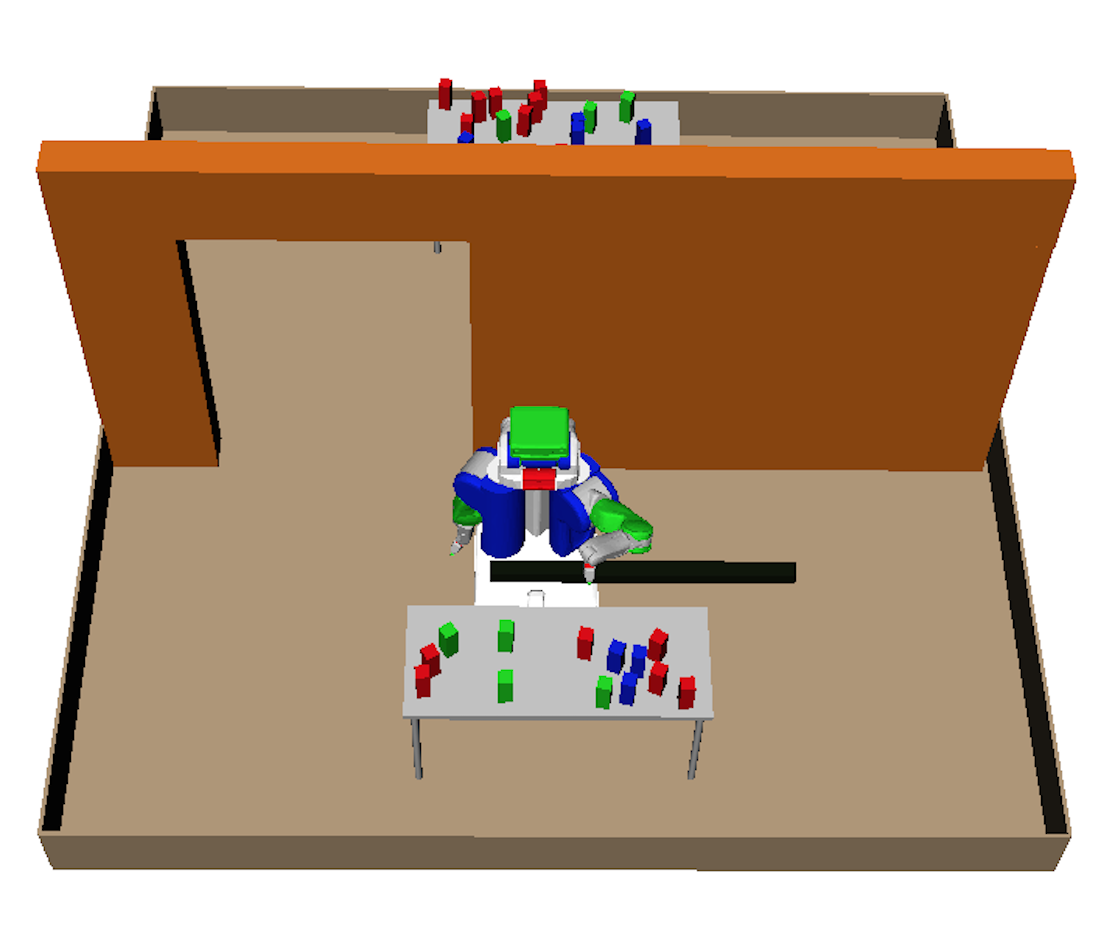
\includegraphics[scale=0.21]{./figures/motivation/1.png}
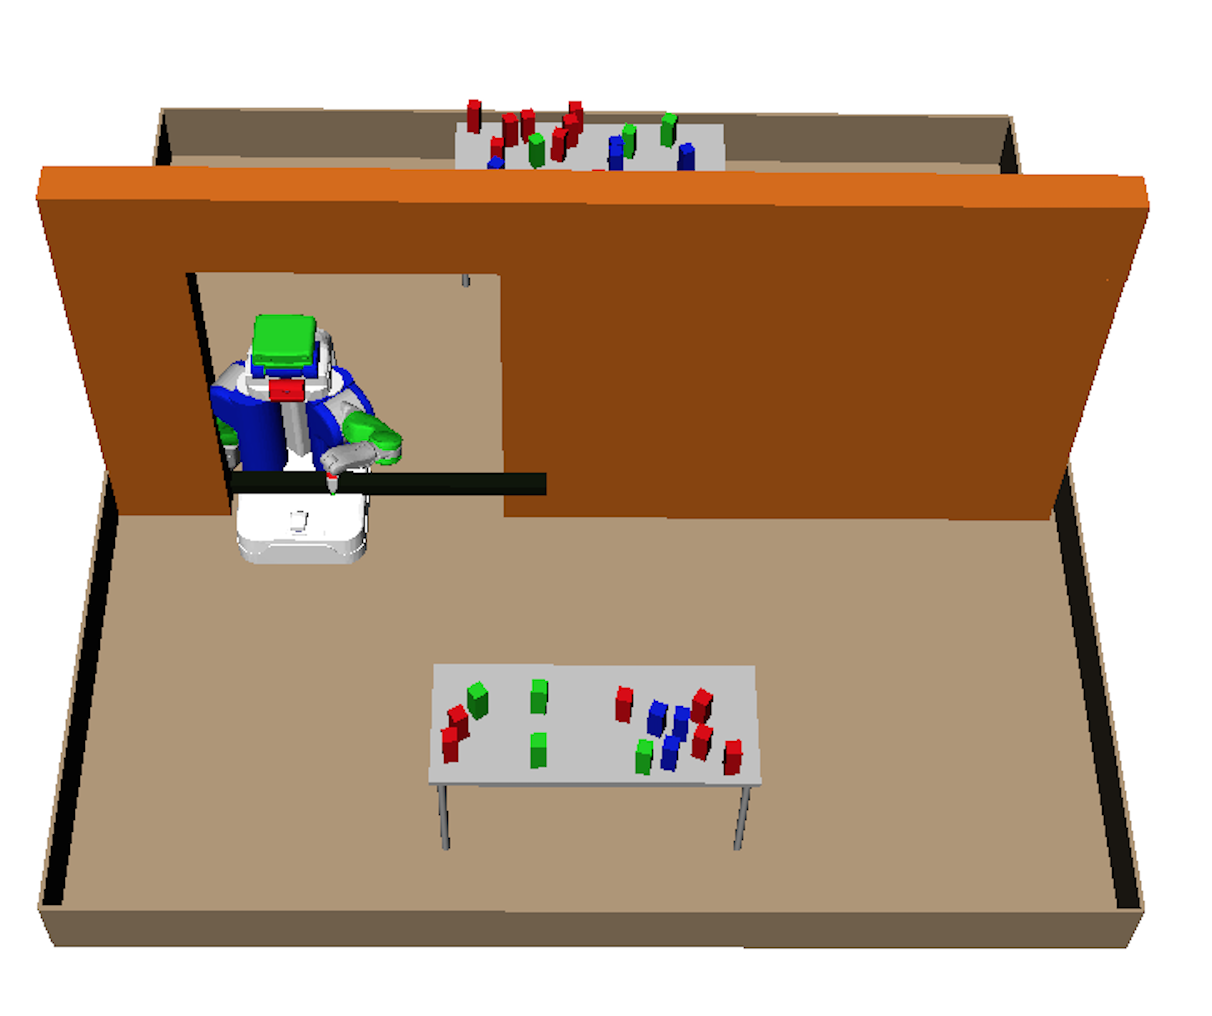
\includegraphics[scale=0.2]{./figures/motivation/3.png}\\
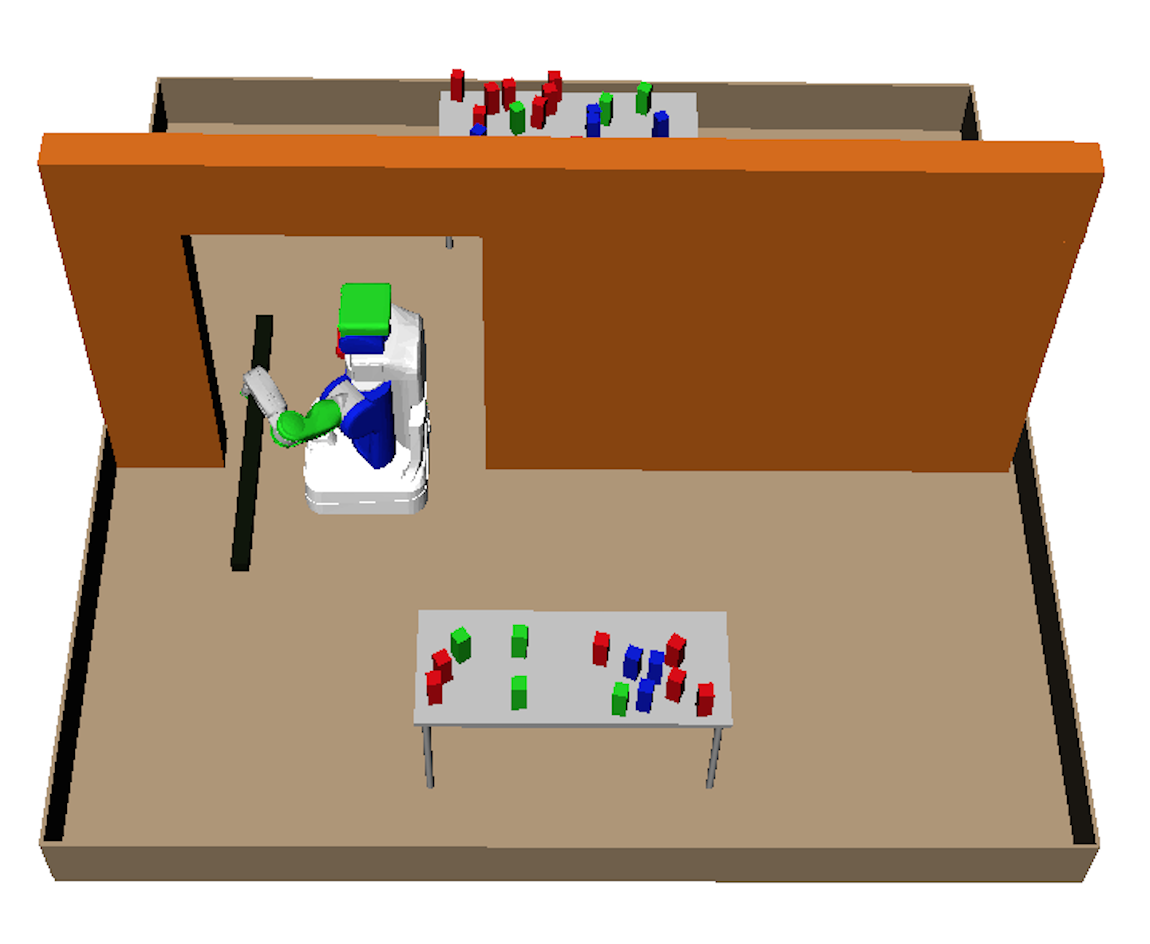
\includegraphics[scale=0.21]{./figures/motivation/4.png}
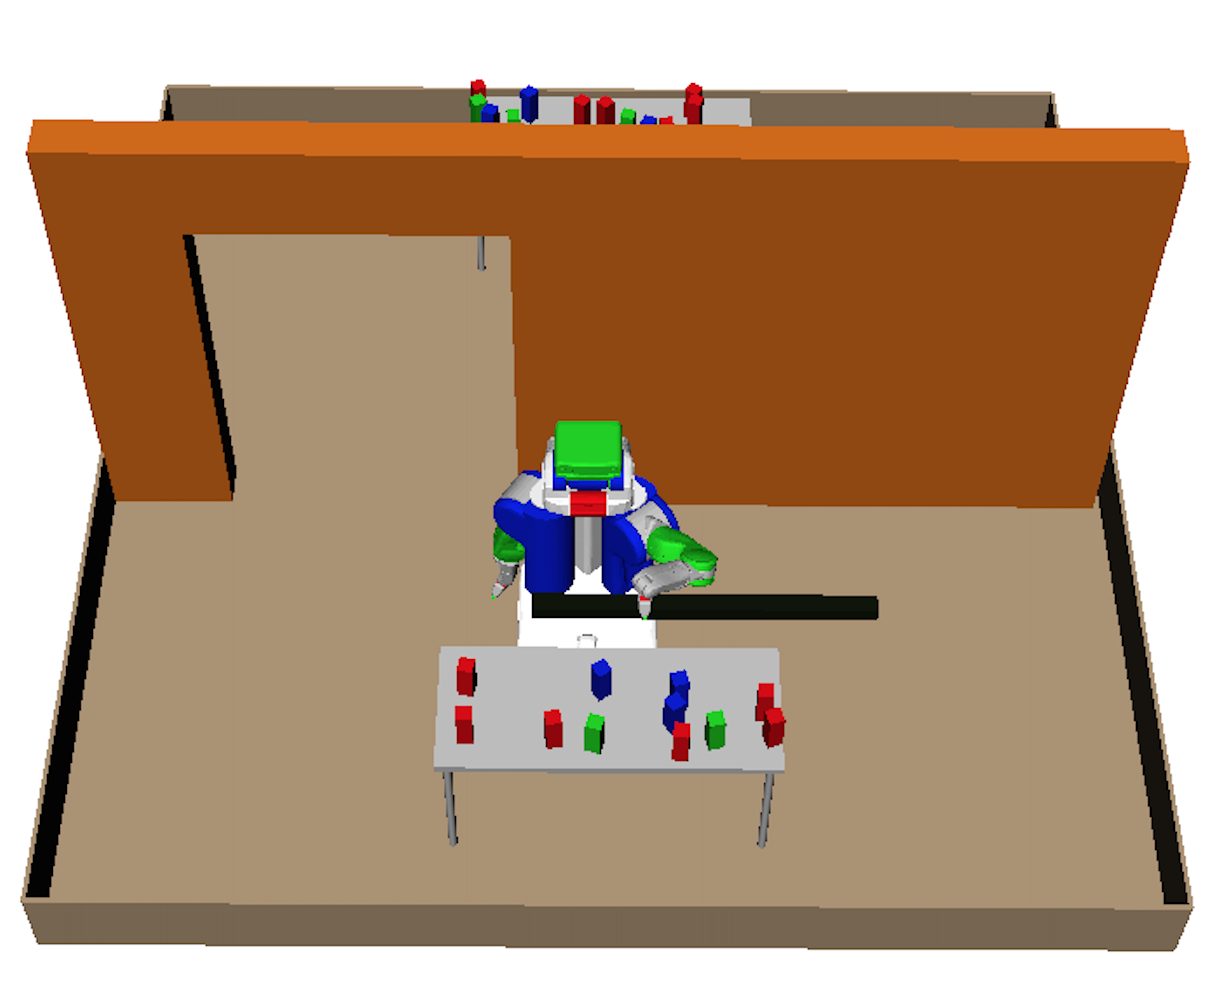
\includegraphics[scale=0.2]{./figures/motivation/2.png}
\caption{ The top two figures in illustrate that this environment
requires you to turn side ways in order to get through the passage, as
shown in bottom left. Bottom right is a new problem instance, with different
arrangement of obstacles on the two tables. Can
we generalize the knowledge that we need to turn side ways from the past problem instance to this one?}
\label{fig:motiv}
\end{figure} 


Current planning algorithms do no try to 
exploit such past knowledge and always plan from scratch.
They spend time on re-doing what it has possibly done before,
which could be used to find a better quality plan. Hence it would
be extremely desirable to be able to adapt such knowledge to
a new planning problem instance intelligently,
as to improve the speed and quality of planning.

In light of this, we introduce the notion of 
\emph{solution contraint} as a representation
 of such past knowledge that informs the 
planner to more quickly generate high quality plans.
A solution constraint could be a
subgoal to quickly plan a motion through a narrow passage,
a grasp to robustly picking an object,
or the closest feasible object pose for placing 
it on a region of interest. We believe
this is more compact and generalizable
representation of past planning knowledge than the 
plans themselves, which does not generalize well
to complex problems that we are considering. Hereafter,
we will refer to a solution constraint as 
constraint whenever trivial from the context.

The main challenge in selecting the best 
solution constraint for the current problem
instance based on the past planning solutions is that 
there is no notion of metric in the space of 
planning problem instances. Instead of constructing
such representation, we directly characterize 
planning problem instances with a library
of solution constraints and their scores in each
of the problems. The main intuition 
here is in viewing the surrounding environment, which defines a 
planning problem instance, as a black box function
which outputs a numerical evaluation of 
the robot's plan associated with the constraint, in lieu of representing
it with some sensory data, which can be misleading.
The relationship between problem instances then can be
constructed based on these values.

More specifically, using this library of solution constraints, we make the
the assumption that the score functions for the problem instances
are sampled from the same distribution. This assumption allows us 
to construct an upper confidence bound (UCB) for the scores
of the new problem instance, using statistics of the past values. 
Based on this bound, we propose BOX (Blackbox Optimization with Experience),
an UCB-type algorithm that tries to find a good solution constraint
for the new scene.

We evaluate the performance BOX in three different domains. In
the first domain, the robot needs to pick an object up by choosing a grasp from
a discrete set. Its objective is to choose the best grasp such that
when the motion planner is constraint to plan a path to the selected pregrasp pose,
the path maximizes the distance from the obstacles. A planning
problem instance is defined by the random arrangement of obstacles.
In the second domain, the robot is faced with the same task, but in addition
to grasp it needs to choose a base pose from a continuous space. A
problem instance is again defined by the arrangement of obstacles.
In the last domain, the robot has to transport an object of random
length from one table to another, where there is a narrow passage in between.
A solution constraint for this domain consists of a grasp for picking
up the object, an object placement pose, robot base pose for
placing the object, and subgoals for motions to pregrasp pose,
to the target base pose, and placement pose. A problem
instance is defined by both the length and arrangement of obstacles. The objective
for this domain is to minimize the sum of the lengths of three paths. 
We compare BOX to four other algorithms, and show that BOX outperforms them both
in terms of time and quality of the plans that it produces in all domains.
